\section{Vorgehen}

\begin{frame}
  \frametitle{Programmaufbau}
\end{frame}
 
 
 
 
 

\begin{frame}
\frametitle{Inverse Kinematik}
\textit{Wie muss die Winkelstellung des Greifarm sein, damit die aktuelle Position der Hand erreicht wird?}\\
\vspace*{1cm}
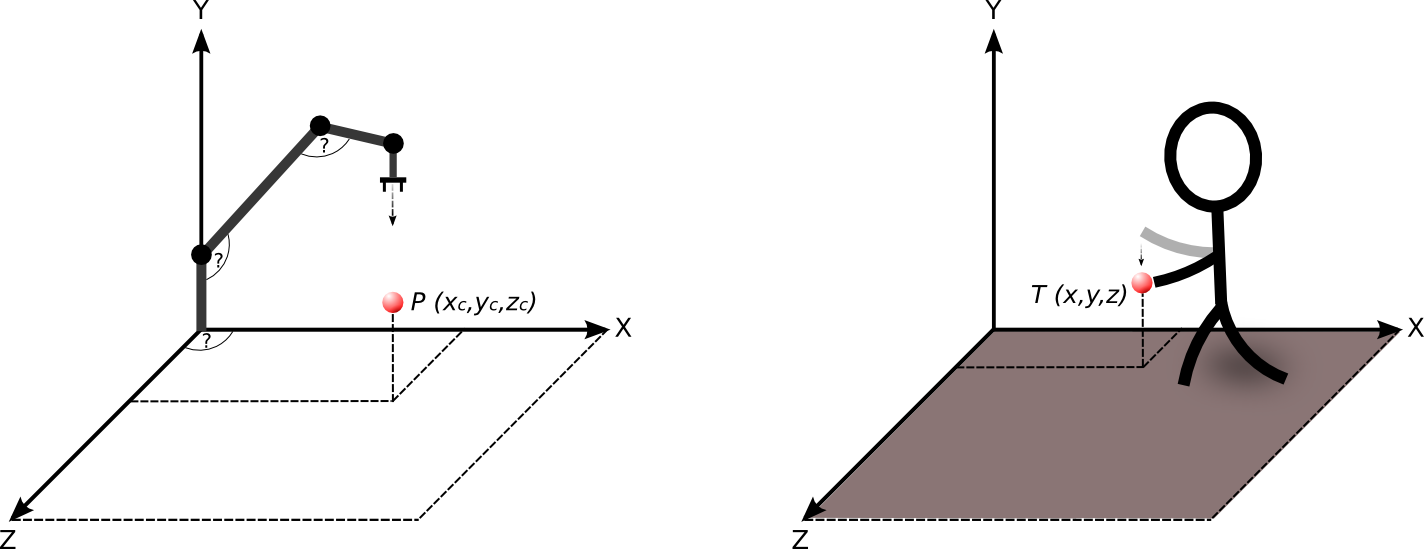
\includegraphics[width=\textwidth]{imgs/kinematikProblem.png}
\end{frame}

\begin{frame}
\frametitle{Inverse Kinematik}
\begin{enumerate}
\item 
\end{enumerate}



\end{frame}



\begin{frame}
  \frametitle{Single-Player Modus}

\end{frame}

\begin{frame}
  \frametitle{Multi-Player Modus}

\end{frame}